\section{Page-Wootters model: \texttt{NN}-level clock $+$ $2$-level system}

\begin{Verbatim}
NN := 32
\end{Verbatim}

\begin{Verbatim}
T := DiagonalMatrix[Range[0,NN-1]]
\end{Verbatim}

\begin{Verbatim}
F := FourierMatrix[NN]
\end{Verbatim}

For simplicity, $\hbar = 1$, there's no ``characteristic frequency'' $\omega$,
and we ignore the dimensional term in front of \eqref{eq:SI_Fourier:T}:

\begin{Verbatim}
\[CapitalOmega] := F.T.F\[ConjugateTranspose] 
\end{Verbatim}

Hamiltonian in "ordinary" space
\begin{Verbatim}
Hs := \[ImaginaryI]{{0, 1}, {-1, 0}}
\end{Verbatim}
\begin{Verbatim}
MatrixForm[Hs]
\end{Verbatim}
\[
  \left(
    \begin{array}{cc}
     0 & i \\
     -i & 0 \\
    \end{array}
    \right)
\]

Matrix representation of \cite[Eq. 1]{Lloyd:Time}.
We turn it into numeric (\verb!N[ ]!) as treating  it symbolically onwards would be unfeasible:
\begin{Verbatim}
J := N[KroneckerProduct[\[CapitalOmega],IdentityMatrix[2]] + KroneckerProduct[IdentityMatrix[NN],Hs]]
\end{Verbatim}
\begin{Verbatim}
Chop[Eigenvalues[J]]

Out[ ] = {32., 31., 30., 30., 29., 29., 28., 28., 27., 27., 26., 26., 25., 25., 24., 24., 23., 23., 22., 22., 21., 21., 20., 20., 19., 19., 18., 18., 17., 17., 16., 16., 15., 15., 14., 14., 13., 13., 12., 12., 11., 11., 10., 10., 9., 9., 8., 8., 7., 7., 6., 6., 5., 5., 4., 4., 3., 3., 2., 2., 1., 1., -1., 0}
\end{Verbatim}
\begin{Verbatim}
Eigenvalues[J][[40]]

Out[ ] = 12.

Eigenvalues[J][[41]]

Out[ ] = 11.

chosenEigenvector := Eigenvectors[J][[ 40]]

chosenEigenvectorB := Eigenvectors[J][[41]]

Normalization := Sqrt[Abs[chosenEigenvector[[1]]^2] + Abs[chosenEigenvector[[2]]^2] ]

NormalizationB := Sqrt[Abs[chosenEigenvectorB[[1]]^2] + Abs[chosenEigenvectorB[[2]]^2] ]

chosenEigenvectorNormalized  := chosenEigenvector / Normalization

chosenEigenvectorNormalizedB := chosenEigenvectorB / NormalizationB  

probability := Abs[chosenEigenvectorNormalized ^2]

probabilityB := Abs[chosenEigenvectorNormalizedB^2]

probability

Out[ ]= {0.716702, 0.283298, 0.771924, 0.228076, 0.785749, 0.214251, 0.756071, 0.243929, 0.687408, 0.312592, 0.590214, 0.409786, 0.479286, 0.520714, 0.371512, 0.628488, 0.283298, 0.716702, 0.228076, 0.771924, 0.214251, 0.785749, 0.243929, 0.756071, 0.312592, 0.687408, 0.409786, 0.590214, 0.520714, 0.479286, 0.628488, 0.371512, 0.716702, 0.283298, 0.771924, 0.228076, 0.785749, 0.214251, 0.756071, 0.243929, 0.687408, 0.312592, 0.590214, 0.409786, 0.479286, 0.520714, 0.371512, 0.628488, 0.283298, 0.716702, 0.228076, 0.771924, 0.214251, 0.785749, 0.243929, 0.756071, 0.312592, 0.687408, 0.409786, 0.590214, 0.520714, 0.479286, 0.628488, 0.371512}

probabilityB

Out[ ]= {0.881533, 0.118467, 0.744511, 0.255489, 0.570264, 0.429736, 0.38532, 0.61468, 0.217835, 0.782165, 0.0933066, 0.906693, 0.0306941, 0.969306, 0.0395291, 0.960471, 0.118467, 0.881533, 0.255489, 0.744511, 0.429736, 0.570264, 0.61468, 0.38532, 0.782165, 0.217835, 0.906693, 0.0933066, 0.969306, 0.0306941, 0.960471, 0.0395291, 0.881533, 0.118467, 0.744511, 0.255489, 0.570264, 0.429736, 0.38532, 0.61468, 0.217835, 0.782165, 0.0933066, 0.906693, 0.0306941, 0.969306, 0.0395291, 0.960471, 0.118467, 0.881533, 0.255489, 0.744511, 0.429736, 0.570264, 0.61468, 0.38532, 0.782165, 0.217835, 0.906693, 0.0933066, 0.969306, 0.0306941, 0.960471, 0.0395291}

ListPlot[probability,
  GridLines ->{Range[0,NN*2, 2], Range[0, 1, 0.1]},
  AxesLabel->{n, "P(0), P(1)"},
  LabelStyle->Directive[16],
  PlotMarkers->{Automatic, 16},
  ImageSize->1024
]
\end{Verbatim}
\begin{figure}[!h]
  \centering
  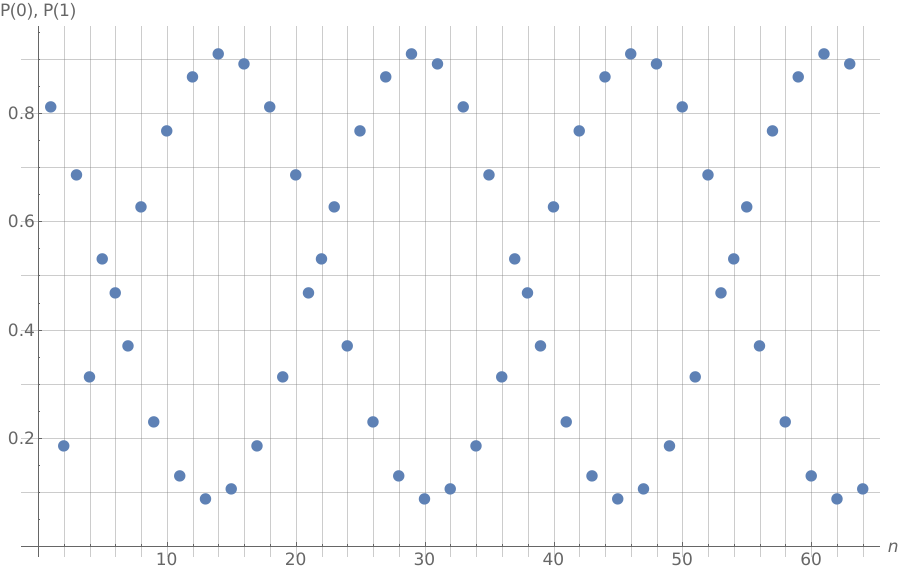
\includegraphics[width=.75\textwidth]{img/N32.png}
  \caption[(from notebook)]{P-W ``evolution'' for $\hat{\mathbb{J}}$ eigenvalue $=12$}
\end{figure}  
\begin{Verbatim}

ListPlot[probabilityB,
  GridLines ->{Range[0,NN*2, 2], Range[0, 1, 0.1]},
  AxesLabel->{n, "P(0), P(1)"},
  LabelStyle->Directive[16],
  PlotMarkers->{Automatic, 16},
  ImageSize->1024
]
\end{Verbatim}
\begin{figure}[!h]
  \centering
  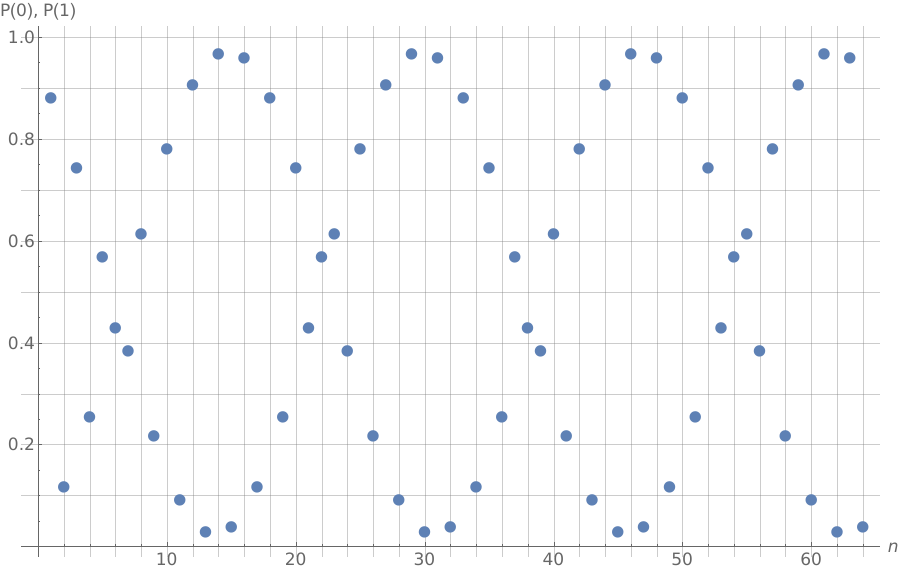
\includegraphics[width=.75\textwidth]{img/N32-B.png}
  \caption[(from notebook)]{P-W ``evolution'' for $\hat{\mathbb{J}}$ eigenvalue $=11$}
\end{figure}

\subsection{Consistency of PW with ordinary QM (discrete approximation)}

\begin{Verbatim}
psi0 :=  chosenEigenvectorNormalizedB[[{1,2}]]

psi0

Out[ ] = {-0.938878+0.00640243 I,0.299377 -0.169824 I}
\end{Verbatim}

\begin{Verbatim}
psi[t_] := MatrixExp[-I Hs t, psi0 ]

psi[t]

{(-0.938878+0.00640243 I) Cos[t]+(0.299377 -0.169824 I) Sin[t],(0.299377 -0.169824 I) Cos[t]+(0.938878 -0.00640243 I) Sin[t]}
\end{Verbatim}

\begin{Verbatim}
(Abs[psi[t]]^2)[[1]]

Out[ ] = Abs[(-0.938878+0.00640243 I) Cos[t]+(0.299377 -0.169824 I) Sin[t]]^2

Plot[Abs[(-0.938878+0.00640243 I) Cos[t]+(0.299377 -0.169824 I) Sin[t]]^2, {t,0,2\[Pi]}
  AxesLabel->{t, "P(0"},
  LabelStyle->Directive[16],
  ImageSize->900
]
\end{Verbatim}
\begin{figure}[!h]
  \centering
  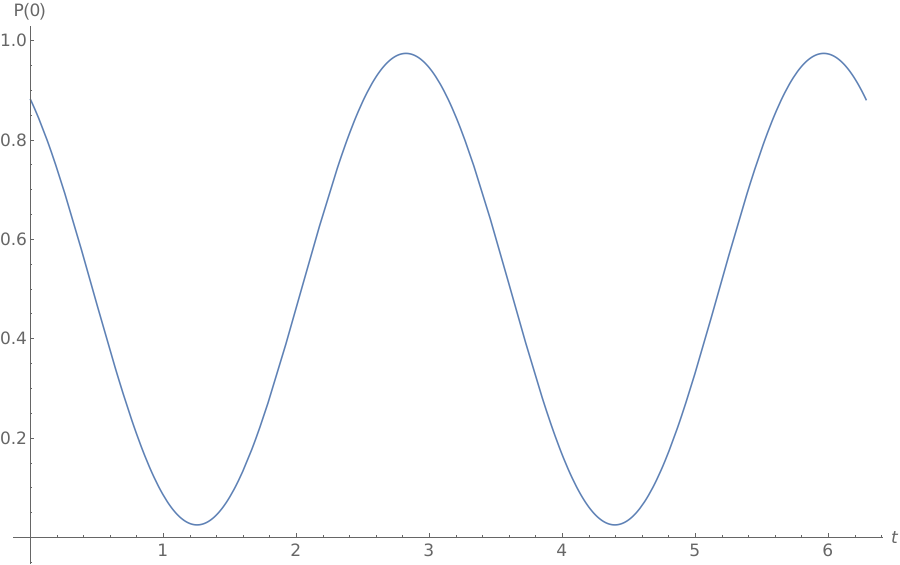
\includegraphics[width=0.75\textwidth]{img/probB_0.png}
  \caption[(from notebook)]{
    Schr{\"o}dinger evolution of
    $\qty|\braket{0}{\psi(t)}|^2$, $t \in (0, 2\pi) $
    picking the first two components of an eigenvector of $\hat{\mathbb{J}}$
    as the two components of $\psi_{t=0}$ in ordinary Hilbert space.
    Related eigenvalue of $\hat{\mathbb{J}}$ is $11$
  }
\end{figure}

\begin{Verbatim}
(Abs[psi[t]]^2)[[2]]

Out[ ] = Abs[(0.299377 -0.169824 I) Cos[t]+(0.938878 -0.00640243 I) Sin[t]]^2
  
Plot[Abs[(0.299377 -0.169824 I) Cos[t]+(0.938878 -0.00640243 I) Sin[t]]^2, {t,0,2\[Pi]}
  AxesLabel->{t, "P(0"},
  LabelStyle->Directive[16],
  ImageSize->900
]
\end{Verbatim}
\begin{figure}[!h]
  \centering
  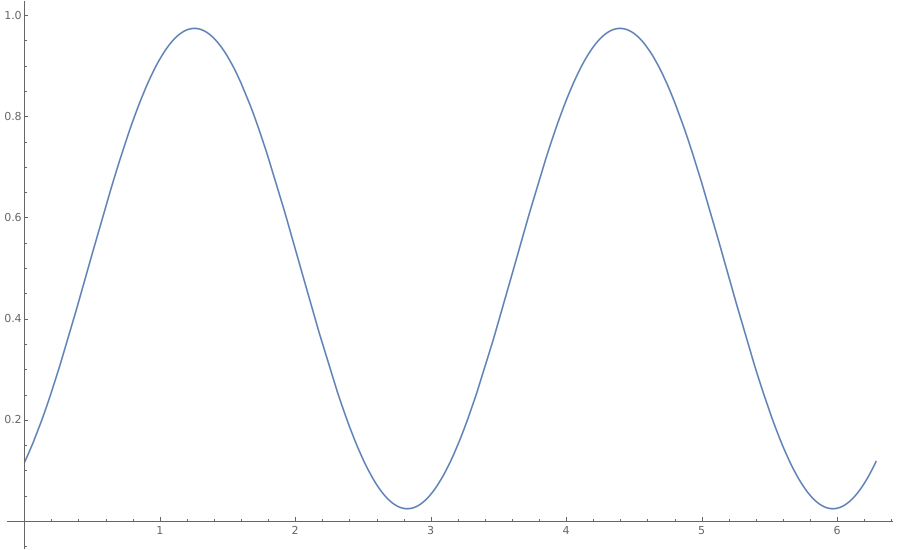
\includegraphics[width=0.75\textwidth]{img/probB_1.png}
  \caption[(from notebook)]{
    Schr{\"o}dinger evolution of
    $\qty|\braket{1}{\psi(t)}|^2$, $t \in (0, 2\pi) $
    picking the first two components of an eigenvector of $\hat{\mathbb{J}}$
    as the two components of $\psi_{t=0}$ in ordinary Hilbert space.
    Related eigenvalue of $\hat{\mathbb{J}}$ is $11$
  }
\end{figure}

\subsubsection{Complex evolution of $\psi$ (not just $\qty|\psi|^2$)}
\begin{Verbatim}
psi[t][[1]]

Out[ ] = (-0.938878 +0.00640243 \[ImaginaryI]) Cos[t] + (0.299377 - 0.169824 \[ImaginaryI]) Sin[t]
\end{Verbatim}
\begin{Verbatim}
psi[t][[2]]

Out[ ]= (0.299377 -0.169824 \[ImaginaryI]) Cos[t] + (0.938878 -0.00640243 \[ImaginaryI]) Sin[t]
\end{Verbatim}  
Real and imaginary part: let's do this manually ---please note index count is
$1, 2$ (cells above)
but refers, respectively, to computational base elements
$\ket{0}, \ket{1}$ in ordinary Hilbert space.
\begin{Verbatim}
re0psi[t_] := (-0.938878) Cos[t]  + (0.299377) Sin[t]
im0psi[t_] := (0.00640243) Cos[t] + (- 0.169824 ) Sin[t]
re1psi[t_] := (0.299377) Cos[t]   + (0.938878) Sin[t]
im1psi[t_] := (- 0.169824) Cos[t] + (- 0.00640243) Sin[t] 
\end{Verbatim}

\begin{Verbatim}
zAxis := ParametricPlot3D[{0,0,t}, {t,0,2\[Pi]}, PlotStyle->{Gray}]
psi0plot := ParametricPlot3D[{re0psi[t], im0psi[t], t}, {t, 0, 2\[Pi]}, PlotStyle->{Red} ]
psi1plot := ParametricPlot3D[{re1psi[t], im1psi[t], t}, {t, 0, 2\[Pi]}, PlotStyle->{Blue} ]
\end{Verbatim}

\begin{Verbatim}
Show[zAxis, psi0plot,psi1plot, ImageSize->Medium,
  AxesLabel -> {
    Style[Re["<0,1|\[Psi]>"], Bold],
    Style[Im["<0,1|\[Psi]>"], Bold],
    Style[t, Bold]
  }
]
\end{Verbatim}
\begin{figure}[!h]
  \centering
  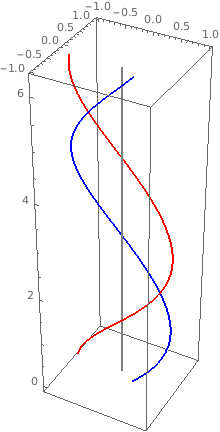
\includegraphics[width=0.25\textwidth]{img/qubit-evo-schrod.png}
  \caption[(from notebook)]{
    Schr{\"o}dinger full complex evolution of components
    $\braket{0}{\psi(t)}$ (red) and 
    $\braket{1}{\psi(t)}$ (blue) for
    $t \in (0, 2\pi) $. The initial state
    has been chosen as the first two components of an eigenstate of
    $\hat{\mathbb{J}}$, related to eigenvalue $= 11$.
  }
\end{figure}

\begin{Verbatim}
pi = N[\[Pi]]

3.14159
\end{Verbatim}

\begin{Verbatim}
rephased[k_] := chosenEigenvectorNormalizedB [[k]] * Exp[-\[ImaginaryI]*pi*11*(k-1)/NN]

rephased1[k_] := chosenEigenvectorNormalizedB [[k]] * Exp[-\[ImaginaryI]*pi*11*(k-2)/NN]

scatter[k_] := {Re[ rephased[k]], Im[ rephased[k]], pi*(k-1)/NN}

scatter1[k_] := {Re[ rephased1[k]], Im[ rephased1[k]], pi*(k-2)/NN}

scatterPoints = Map[scatter, Range[1,2*NN, 2]]

Out[ ] = {{-0.938878,0.00640243,0.}, {-0.862432,-0.0268517,0.19635}, {-0.752844,-0.0590739,0.392699}, {-0.614324,-0.089026,0.589049}, {-0.452196,-0.115557,0.785398}, {-0.27269,-0.137647,0.981748}, {-0.0827052,-0.154447,1.1781}, {0.110458,-0.165312,1.37445}, {0.299377,-0.169824,1.5708}, {0.47679,-0.16781,1.76715}, {0.635881,-0.159347,1.9635}, {0.770535,-0.144761,2.15984}, {0.875578,-0.124611,2.35619}, {0.946973,-0.0996728,2.55254}, {0.981977,-0.0709041,2.74889}, {0.979243,-0.0394105,2.94524}, {0.938878,-0.00640243,3.14159}, {0.862432,0.0268517,3.33794}, {0.752844,0.0590739,3.53429}, {0.614324,0.089026,3.73064}, {0.452196,0.115557,3.92699}, {0.27269,0.137647,4.12334}, {0.0827052,0.154447,4.31969}, {-0.110458,0.165312,4.51604}, {-0.299377,0.169824,4.71239}, {-0.47679,0.16781,4.90874}, {-0.635881,0.159347,5.10509}, {-0.770535,0.144761,5.30144}, {-0.875578,0.124611,5.49779}, {-0.946973,0.0996728,5.69414}, {-0.981977,0.0709041,5.89049}, {-0.979243,0.0394105,6.08684}}

scatterPoints1 = Map[scatter1, Range[2,2*NN, 2]]

Out[ ] = {{0.299377,-0.169824,0.}, {0.47679,-0.16781,0.19635}, {0.635881,-0.159347,0.392699}, {0.770535,-0.144761,0.589049}, {0.875578,-0.124611,0.785398}, {0.946973,-0.0996728,0.981748}, {0.981977,-0.0709041,1.1781}, {0.979243,-0.0394105,1.37445}, {0.938878,-0.00640243,1.5708}, {0.862432,0.0268517,1.76715}, {0.752844,0.0590739,1.9635}, {0.614324,0.089026,2.15984}, {0.452196,0.115557,2.35619}, {0.27269,0.137647,2.55254}, {0.0827052,0.154447,2.74889}, {-0.110458,0.165312,2.94524}, {-0.299377,0.169824,3.14159}, {-0.47679,0.16781,3.33794}, {-0.635881,0.159347,3.53429}, {-0.770535,0.144761,3.73064}, {-0.875578,0.124611,3.92699}, {-0.946973,0.0996728,4.12334}, {-0.981977,0.0709041,4.31969}, {-0.979243,0.0394105,4.51604}, {-0.938878,0.00640243,4.71239}, {-0.862432,-0.0268517,4.90874}, {-0.752844,-0.0590739,5.10509}, {-0.614324,-0.089026,5.30144}, {-0.452196,-0.115557,5.49779}, {-0.27269,-0.137647,5.69414}, {-0.0827052,-0.154447,5.89049}, {0.110458,-0.165312,6.08684}}
\end{Verbatim}

\begin{Verbatim}
scatterPlot = ListPointPlot3D[scatterPoints, PlotStyle->{Red, PointSize[Large]}]
\end{Verbatim}
\begin{figure}[!h]
  \centering
  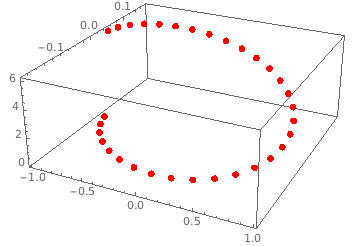
\includegraphics[width=0.4\textwidth]{img/scatterplot0.png}
  \caption[(from notebook)]{
    Page-Wootters discrete-time evolution of
    $\braket{0}{\psi(t)}$ in 32 points between
    $t \in (0, 2\pi) $. From an eigenstate of
    $\hat{\mathbb{J}}$ related to eigenvalue $\epsilon = 11$.
    The evolution has been ``corrected'' via a phase oscillation
    factor $e^{-i \epsilon t}$
    as explained in \cite[``The Zero-eigenvalue'']{Lloyd:Time}.
  }
\end{figure}

\begin{Verbatim}
scatterPlot1 = ListPointPlot3D[scatterPoints1, PlotStyle->{Blue, PointSize[Large]}]
\end{Verbatim}
\begin{figure}[!h]
  \centering
  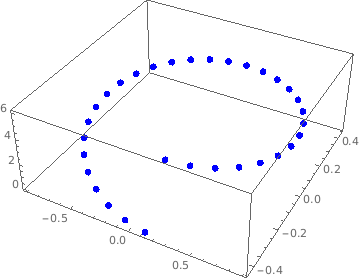
\includegraphics[width=0.4\textwidth]{img/scatterplot1.png}
  \caption[(from notebook)]{
    Page-Wootters discrete-time evolution of
    $\braket{1}{\psi(t)}$ in 32 points between
    $t \in (0, 2\pi) $. From an eigenstate of
    $\hat{\mathbb{J}}$ related to eigenvalue $\epsilon = 11$.
    The evolution has been ``corrected'' via a phase oscillation
    factor $e^{-i \epsilon t}$
    as explained in \cite[``The Zero-eigenvalue'']{Lloyd:Time}.
  }
\end{figure}

\begin{Verbatim}
Show[zAxis, psi0plot,psi1plot,scatterPlot, scatterPlot1, ImageSize->Large]
\end{Verbatim}
\begin{figure}[!h]
  \centering
  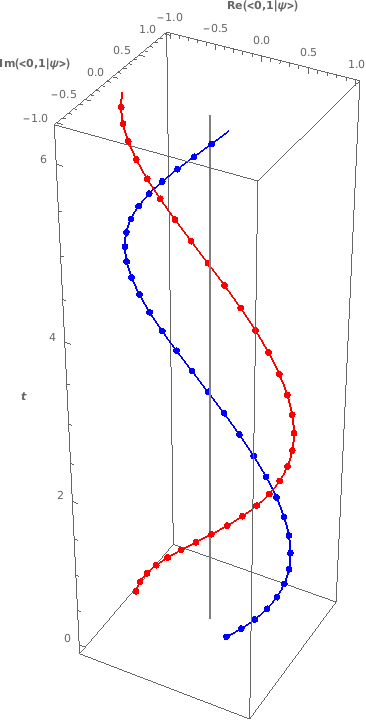
\includegraphics[width=0.4\textwidth]{img/PWfit32.png}
  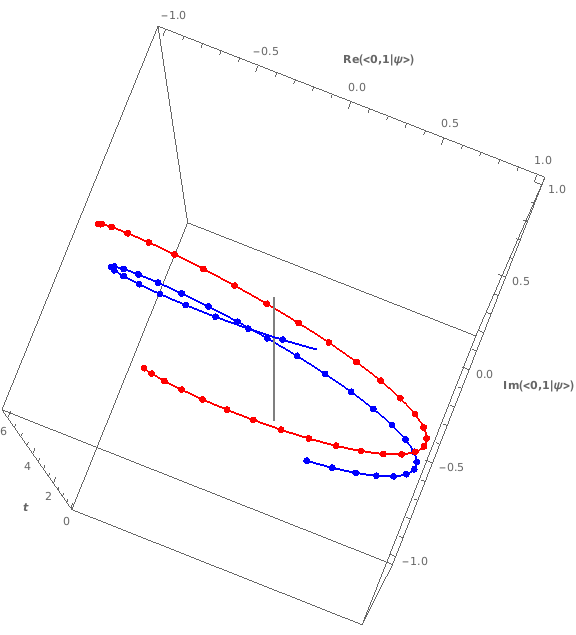
\includegraphics[width=0.6\textwidth]{img/PWfit32top.png}
  \caption[(from notebook)]{
    Page-Wootters discrete-time ``evolution without evolution'' (points)
    is interpolated by the (continuous lines) of standard quantum mechanics
    evolution ---up to a suitable phase correction, as seen previously.
    Horizontal axis are real and imaginary part of the wave function components.
    Vertical axis is time. 
  }
\end{figure}
